\chapter{Probleemanalyse}

\section{Probleemomschrijving}
Het project heet Satellite. Satellite is een nieuw project dat ontwikkeld wordt door Sensor Maritime in het kader van sensor data gedreven optimalisatie voor scheepvaart. Het geeft een kapitein de mogelijkheid om aan de hand van data kosten te besparen. Dit wordt gedaan door gegevens te verzamelen. Met deze data kan een kapitein efficiënter werken door veiliger, slimmer en duurzamer te opereren. Elke kapitein zal andere data willen voor zijn binnenvaartschip. Dit betekent dat het veranderen van sensoren simpel en snel moet zijn. Satellite (zie \ref{fig:shw} is zo ontwikkeld dat je plug \& play verschillende sensoren kan toevoegen. Dit wordt gedaan door verschillende IO porten en connectors toe te voegen aan de hardware. De Satellite hardware is al ontwikkeld, maar mist alleen nog de software om het als product te gebruiken. Aan de afstudeerder is  gevraagd om voor de hardware de applicatie te schrijven. Er moet nadruk gelegd worden bij de oplevering dat er een robuust en een generieke applicatie ontwikkeld wordt, die gefocust is op zowel de klant als de ontwikkelaar. Vervolgens is er ook gevraagd aan de afstudeerder om een systeem op te zetten dat toekomstige Satellite hardware snel en makkelijk getest kan worden.
\begin{figure}[h!]
	\begin{centering}

	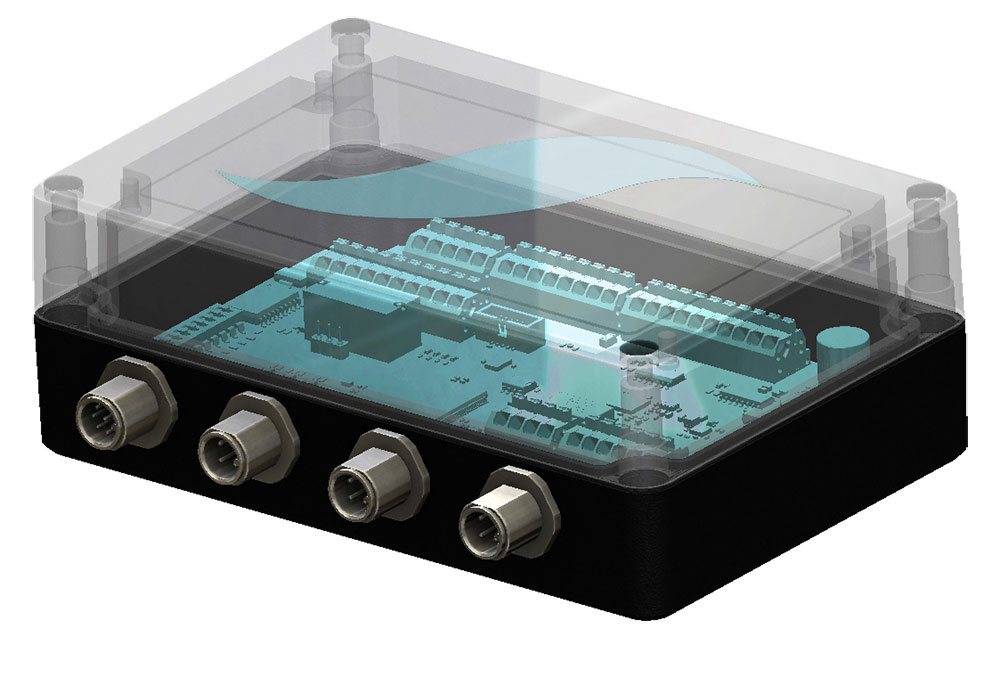
\includegraphics[width=0.35\linewidth]{statements/satellite.jpg}
	\caption{Satellite hardware}
	\label{fig:shw}
	\end{centering}
\end{figure}

\section{Betrokken partijen}
Tijdens de afstudeerstage zijn er twee partijen betrokken, Sensor Maritime in Vught en de student die de afstudeerstage volgt. Mark-Ivo van Ooijen van Sensor Maritime is de begeleider en projectleider. De tweede partij is de afstudeerder zelf, Patrick de Jong. Vanuit school zijn er ook twee examinatoren, maar deze zijn niet betrokken bij het project zelf. De examinatoren zijn Andries van Dongen, hij is de docentbegeleider die de afstudeerstage zal begeleiden. Pieter Kop Jansen zal er alleen zijn bij de uiteindelijke verdediging.

\section{Onderzoeksvraag}
De onderzoeksvraag tijdens de afstudeerstage is: \textbf{hoe kan een modulair softwaresysteem worden ontwikkeld voor de Satellite hardware zo dat verschillende sensoren ondersteund worden en data verstuurd kan worden naar één hoofdsysteem?}

\section{Deelvragen}
Het systeem moet robuust en makkelijk uitbreidbaar zijn. Daar sluiten dan twee van de deelvragen op aan. Bij een deelvraag is er gekeken naar de hardware validatie. Dit is een extra onderdeel wat Sensor Maritime aan de afstudeerder heeft gevraagd om een manier te ontwikkelen zodat er makkelijk nieuwe Satellite hardware getest kan worden.
\begin{enumerate}
	\item Hoe kan er een robuuste  communicatie gecreëerd worden tussen een hoofdsysteem en Satellite?
	\item Op welke manier moet de software ontworpen worden zodat het makkelijk uitbreidbaar is met nieuwe sensoren?
	\item Welke stappen zijn nodig om alle IO porten te testen van de Satellite?
\end{enumerate}

\section{Doelstellingen}
De doelstellingen van het project geven duidelijkheid in wat er precies bereikt moet worden in betrekking met de onderzoeksvraag en deelvraag. Dit is de lijst die de te bereiken doelstellingen aangeeft.
\begin{enumerate}
	\item De Satellite IO porten zijn volledig getest, en kunnen communiceren met sensoren.
	\item De Satellite heeft een robuuste communicatie over CAN en UDP. 
	\item De Satellite werkt met generieke en modulair opgebouwde software, waardoor het product in de toekomst makkelijk uitgebreid kan worden.
\end{enumerate}

\newpage
\section{Eisen}
Voor dat er een applicatie ontwikkeld kon worden is er besproken met de stagebegeleider waar de applicatie aan moet voldoen. De volgende tabel \ref{tab:eisen} geeft een overzicht van de eisen voor het project Satellite.
\begin{table}[h!]
	\centering
	\caption{MoSCoW Analyse}
	\label{tab:eisen}
	\begin{tabular}{lp{13cm}l}
	\toprule
	\textbf{ID} & \textbf{Eis} & \textbf{Prioriteit} \\ \midrule
	SM1			& Alle IO porten van de Satellite moeten getest worden 										& MUST	 \\
	SM2			& Implementatie van de hoekmeting en versnellingsassen 										& MUST	 \\ 
	SM3			& Spectrum analyse maken van de versnellingsassen 											& MUST	 \\ 
	SM4			& Errors moeten goed afgevangen worden, de applicatie mag niet crashen of blijven hangen 	& MUST	 \\ 
	SM5			& CAN-implementatie, en correct protocol afhandeling										& MUST	 \\ \midrule
	SM6			& Implementatie voor IO-Link sensoren 														& SHOULD \\
	SM7			& Hoogte sensoren en antenne sensor inlezen 												& SHOULD \\  \midrule
	SM8			& Standaard datastructuur voor packets die worden opgestuurd								& COULD	 \\
	SM9			& Debug berichten worden opgestuurd via UDP/CAN 											& COULD	 \\  \midrule
	SM10		& Ondersteuning van niet gekozen sensoren van Sensor Maritime 								& WON'T	 \\
	SM11		& Ondersteuning voor andere communicatiemiddelen dan UDP, CAN 								& WON'T	 \\
	SM12		& Ondersteuning voor andere embedded systemen  												& WON'T	 \\\bottomrule
	\end{tabular}
\end{table}
